\documentclass[10pt,handout,hyperref={unicode}]{beamer}
%-------------------------------------------------------
% Beamer Theme location override
%-------------------------------------------------------

\makeatletter
  \def\beamer@calltheme#1#2#3{%
    \def\beamer@themelist{#2}
    \@for\beamer@themename:=\beamer@themelist\do%
    {\usepackage[{#1}]{\beamer@themelocation/#3\beamer@themename}}}

  \def\usefolder#1{
    \def\beamer@themelocation{#1}
  }
  \def\beamer@themelocation{}

%-------------------------------------------------------
% INCLUDE PACKAGES
%-------------------------------------------------------

\usepackage{minted} % Code listing
\usepackage{forest} % Tree graphs
\usepackage{fontspec} % UTf-8 input support lualatex
% \usepackage{multirow}
\usepackage{hyperref}
\usepackage{wasysym}
\usepackage[absolute,overlay]{textpos}
\usepackage{graphicx}
\usepackage{microtype} % nice text appearance
\usepackage{ragged2e}
\usepackage{pgfpages}
\usepackage[ngerman]{babel} % german text standards
\usepackage{docmute} % Import other .tex files ignoring document
\usepackage{multicol} % Automatically use multiple columns
\usepackage{fontawesome} % WebFonts including href icon

%-------------------------------------------------------
% Config Theme
%-------------------------------------------------------
\usefolder{../Templates/featherZR}

\usetheme[
    progressstyle=movingCircCnt   % fixedCircCnt, movingCircCnt (moving is deault)
  ]{Feather}

\setsansfont{HelveticaNeue}
\setmonofont{Source Code Pro for Powerline}[Scale = MatchLowercase]

%-------------------------------------------------------
% DEFINING AND REDEFINING COMMANDS
%-------------------------------------------------------

% \setbeameroption{show notes}
% \setbeameroption{show notes on second screen=right}

%Set Path to images
\graphicspath{{Images/}}

% colored hyperlinks
\newcommand{\chref}[2]{%
\href{#1}{{\usebeamercolor[bg]{Feather}#2} {\footnotesize\faExternalLink}}%
}

%Justification
\addtobeamertemplate{theorem begin}{}{\justifying}
\addtobeamertemplate{block begin}{}{\justifying}
\addtobeamertemplate{itemize begin}{}{\justifying}
\addtobeamertemplate{item begin}{}{\justifying}
\addtobeamertemplate{frame begin}{}{\justifying}
\addtobeamertemplate{quote begin}{}{\justifying}
\addtobeamertemplate{structure begin}{}{\justifying}

%etoolbox für nested list covering
\setbeamercovered{transparent}

%description inde
\setbeamersize{description width=0.57cm}

\makeatletter
\newcommand*\fix@beamer@close{%
  \ifnum\beamer@trivlistdepth>0
  \beamer@closeitem%
  \fi
}
\newcommand*\fix@beamer@open{%
  \ifnum\beamer@trivlistdepth>0
  \gdef\beamer@closeitem{}%
  \fi
}
\newcommand<>{\highlighton}[1]{%
  \alt#2{\structure{#1}}{{#1}}
}

\BeforeBeginEnvironment{enumerate}{\fix@beamer@close}
\AfterEndEnvironment{enumerate}{\fix@beamer@open}
\BeforeBeginEnvironment{itemize}{\fix@beamer@close}
\AfterEndEnvironment{itemize}{\fix@beamer@open}
\BeforeBeginEnvironment{description}{\fix@beamer@close}
\AfterEndEnvironment{description}{\fix@beamer@open}
\makeatother

% Codelistings
\definecolor{monokaibg}{HTML}{002833}
\definecolor{highlightbg}{HTML}{004550}

\setminted{
  autogobble=true,
  bgcolor=monokaibg,
  breaklines=true,
  fontsize=\footnotesize,
  highlightcolor=highlightbg,
  linenos=true,
  labelposition=bottomline,
  rulecolor=white,
  style=native,
}

\setmintedinline{
  bgcolor={},
  fontsize=\normalsize,
  style=manni
}

%-------------------------------------------------------
% INFORMATION IN THE TITLE PAGE
%-------------------------------------------------------

\title[PHPUnit Tutorial ] % [] is optional - is placed on the bottom of the sidebar on every slide
{ % is placed on the title page
      \textbf{PHPUnit Tutorial}
}

\subtitle[ -- Funktionsweise von PHPUnit]
{
%      \textbf{v. 1.0.0}
}

\author[Sebastian Knott]{Sebastian Knott}

\institute[]
{
      ZooRoyal IT\\

  %there must be an empty line above this line - otherwise some unwanted space is added between the university and the country (I do not know why;( )
}

\date{\today}

\begin{document}

\documentclass[10pt,hyperref={unicode}]{beamer}

%!TeX spellcheck = en-US,de-DE

%-------------------------------------------------------
% Beamer Theme location override
%-------------------------------------------------------

\makeatletter
  \def\beamer@calltheme#1#2#3{%
    \def\beamer@themelist{#2}
    \@for\beamer@themename:=\beamer@themelist\do
    {\usepackage[{#1}]{\beamer@themelocation/#3\beamer@themename}}}

  \def\usefolder#1{
    \def\beamer@themelocation{#1}
  }
  \def\beamer@themelocation{}

%-------------------------------------------------------
% INCLUDE PACKAGES
%-------------------------------------------------------

\usepackage{minted} % Code listing
\usepackage{forest} % Tree graphs
\usepackage{fontspec} % UTf-8 input support lualatex
% \usepackage{multirow}
\usepackage{hyperref}
\usepackage{wasysym}
\usepackage[absolute,overlay]{textpos}
\usepackage{graphicx}
\usepackage{microtype} % nice text appearance
\usepackage{ragged2e}
\usepackage{pgfpages}
\usepackage[ngerman]{babel} % german text standards
\usepackage{docmute} % Import other .tex files ignoring document
\usepackage{multicol} % Automatically use multiple columns
\usepackage{fontawesome} % WebFonts including href icon

%-------------------------------------------------------
% Config Theme
%-------------------------------------------------------
\usefolder{../Templates/featherZR}
\usetheme[
    progressstyle=movingCircCnt   % fixedCircCnt, movingCircCnt (moving is deault)
  ]{Feather}

\setsansfont{HelveticaNeue}
\setmonofont{Source Code Pro for Powerline}[Scale = MatchLowercase]

%-------------------------------------------------------
% DEFINING AND REDEFINING COMMANDS
%-------------------------------------------------------

% \setbeameroption{show notes}
% \setbeameroption{show notes on second screen=right}

%Set Path to images
\graphicspath{{Images/}}

% colored hyperlinks
\newcommand{\chref}[2]{%
\href{#1}{{\usebeamercolor[bg]{Feather}#2} {\footnotesize\faExternalLink}}%
}

%Justification
\addtobeamertemplate{theorem begin}{}{\justifying}
\addtobeamertemplate{block begin}{}{\justifying}
\addtobeamertemplate{itemize begin}{}{\justifying}
\addtobeamertemplate{item begin}{}{\justifying}
\addtobeamertemplate{frame begin}{}{\justifying}
\addtobeamertemplate{quote begin}{}{\justifying}
\addtobeamertemplate{structure begin}{}{\justifying}

%etoolbox für nested list covering
\setbeamercovered{transparent}

%description inde
\setbeamersize{description width=0.57cm}

\makeatletter
\newcommand*\fix@beamer@close{%
  \ifnum\beamer@trivlistdepth>0
  \beamer@closeitem
  \fi
}
\newcommand*\fix@beamer@open{%
  \ifnum\beamer@trivlistdepth>0
  \gdef\beamer@closeitem{}%
  \fi
}
\newcommand<>{\highlighton}[1]{%
  \alt#2{\structure{#1}}{{#1}}
}

\BeforeBeginEnvironment{enumerate}{\fix@beamer@close}
\AfterEndEnvironment{enumerate}{\fix@beamer@open}
\BeforeBeginEnvironment{itemize}{\fix@beamer@close}
\AfterEndEnvironment{itemize}{\fix@beamer@open}
\BeforeBeginEnvironment{description}{\fix@beamer@close}
\AfterEndEnvironment{description}{\fix@beamer@open}
\makeatother

% Codelistings
\definecolor{monokaibg}{HTML}{002833}
\definecolor{highlightbg}{HTML}{004550}

\setminted{
  autogobble=true,
  bgcolor=monokaibg,
  breaklines=true,
  fontsize=\footnotesize,
  highlightcolor=highlightbg,
  linenos=true,
  labelposition=bottomline,
  rulecolor=white,
  style=native,
}

\setmintedinline{
  bgcolor={},
  fontsize=\normalsize,
  style=manni
}

%-------------------------------------------------------
% INFORMATION IN THE TITLE PAGE
%-------------------------------------------------------

\title[PHPUnit Tutorial ] % [] is optional - is placed on the bottom of the sidebar on every slide
{ % is placed on the title page
      \textbf{PHPUnit Tutorial}
}

\subtitle[ -- Funktionsweise von PHPUnit]
{
%      \textbf{v. 1.0.0}
}

\author[Sebastian Knott]{Sebastian Knott}

\institute[]
{
      ZooRoyal IT\\

  %there must be an empty line above this line - otherwise some unwanted space is added between the university and the country (I do not know why;( )
}

\date{\today}

%-------------------------------------------------------
% THE TITLE OF THE PRESENTATION
%-------------------------------------------------------

\begin{document}

{\1
\begin{frame}[plain,noframenumbering] % the plain option removes the header from the title page, noframenumbering removes the numbering of this frame only
  \titlepage % call the title page information from above
\end{frame}}

% \AtBeginSection[]
% {
%   \frame<handout:0>
%   {
%     \frametitle{Überblick}
%     \tableofcontents[currentsection,hideothersubsections,sectionstyle=show/shaded,subsectionstyle=show/shaded]
%   }
% }

\AtBeginSection[]
{
  \frame<handout:0>
  {
    \frametitle{Überblick}
    \begin{columns}
      \begin{column}{0.3\textwidth}
        \begin{figure}
          \begin{center}
            \includegraphics[width=0.9\textwidth]{PHPUnit_logo}
          \end{center}
        \end{figure}
      \end{column}
      \begin{column}{0.7\textwidth}
        \begin{multicols}{2}
          \tableofcontents[currentsection,sectionstyle=show/shaded,subsectionstyle=show/shaded,subsubsectionstyle=shaded/shaded/hide]
        \end{multicols}
      \end{column}
    \end{columns}
  }
}

\AtBeginSubsection[]
{
  \frame<handout:0>
  {
    \frametitle{Überblick}
    \begin{columns}
      \begin{column}{0.3\textwidth}
        \begin{figure}
          \begin{center}
            \includegraphics[width=0.9\textwidth]{PHPUnit_logo}
          \end{center}
        \end{figure}
      \end{column}
      \begin{column}{0.7\textwidth}
        \begin{multicols}{2}
          \tableofcontents[currentsection,sectionstyle=show/shaded,subsectionstyle=show/shaded,subsubsectionstyle=shaded/shaded/hide]
        \end{multicols}
      \end{column}
    \end{columns}
  }
}

\AtBeginSubsubsection[]
{
  \frame<handout:0>
  {
    \frametitle{Überblick}
    \begin{columns}[onlytextwidth]
      \begin{column}{0.3\textwidth}
        \begin{figure}
          \begin{center}
            \includegraphics[width=0.9\textwidth]{PHPUnit_logo}
          \end{center}
        \end{figure}
      \end{column}
      \begin{column}{0.7\textwidth}
        \begin{multicols}{2}
          \tableofcontents[currentsection,sectionstyle=show/shaded,subsectionstyle=show/shaded,subsubsectionstyle=show/shaded/hide]
        \end{multicols}
      \end{column}
    \end{columns}
  }
}

%-------------------------------------------------------
% THE BODY OF THE PRESENTATION
%-------------------------------------------------------

\begin{frame}
  \frametitle{Überblick}
  \begin{columns}
    \begin{column}{0.3\textwidth}
      \begin{figure}
        \begin{center}
          \includegraphics[width=0.9\textwidth]{PHPUnit_logo}
        \end{center}
      \end{figure}
    \end{column}
    \begin{column}{0.7\textwidth}
      \begin{multicols}{2}
        \tableofcontents[currentsection,sectionstyle=show,subsectionstyle=show/shaded,subsubsectionstyle=hide]
      \end{multicols}
    \end{column}
  \end{columns}
\end{frame}


\section{Bevor es los geht}
\subsection{Was ist PHPUnit}


\begin{frame}
  \frametitle{\secname}
  \framesubtitle{\subsecname}

  \begin{block}{}
    \begin{quotation}
      PHPUnit is a \chref{https://en.wikipedia.org/wiki/Software_framework}{unit testing framework} for the PHP programming language. It is an instance of the \chref{https://en.wikipedia.org/wiki/XUnit}{xUnit} architecture for unit testing frameworks that originated with \chref{https://en.wikipedia.org/wiki/SUnit}{SUnit} and became popular with \chref{https://en.wikipedia.org/wiki/JUnit}{JUnit}. PHPUnit was created by Sebastian Bergmann and its development is hosted on \chref{https://github.com/sebastianbergmann/phpunit}{GitHub}.
    \end{quotation}
    \flushright{{\em -- \chref{https://de.wikipedia.org/wiki/PHPUnit}{Wikipedia.org}}}
  \end{block}
\end{frame}


\begin{frame}
  \frametitle{\secname}
  \framesubtitle{\subsecname}

  \begin{block}{Zweck}
    \begin{quotation}
      PHPUnit is based on the idea that developers should be able to \alert{find mistakes} in their newly committed code quickly and assert that no \chref{https://en.wikipedia.org/wiki/Regression_testing}{code regression} has occurred in other parts of the code base. Much like other \chref{https://en.wikipedia.org/wiki/Unit_testing}{unit testing frameworks}, PHPUnit uses \chref{https://en.wikipedia.org/wiki/XUnit\#Assertions}{assertions} to verify that the behavior of the specific component - or unit - being tested behaves as expected.
    \end{quotation}

    \flushright{{\em -- \chref{https://de.wikipedia.org/wiki/PHPUnit}{Wikipedia.org}}}
  \end{block}
\end{frame}


\subsection{Vorraussetzungen}


\begin{frame}
  \frametitle{Voraussetzungen}
  \framesubtitle{PHP Interpreter}
  \begin{center}
    \begin{columns}
      \begin{column}{0.25\textwidth}
        \begin{figure}
          
\includegraphics[width=\textwidth]{logo-php}
        \end{figure}
      \end{column}
      \begin{column}{0.75\textwidth}
        \begin{itemize}
          \item Für viele Features wird Xdebug benötigt
          \item Version von PHPUnit hängt von PHP Version ab
        \end{itemize}
      \end{column}
    \end{columns}
    \vspace{2em}
    \begin{figure}
      \begin{center}
        \bgroup
          \def\arraystretch{1.2}
          \begin{tabular}{ c c c c }
            PHPUnit & PHP & Release & Support \\ \hline
            7 &	7.1 -- 7.3 &	2.2.2018 & Ends on 7.2.2020 \\
            6 &	7.0 -- 7.2 &	3.2.2017 & Ends on 1.2.2019 \\
            5 &	5.6 -- 7.0 &	2.10.2015 & Ends on 2.2.2018 \\
          \end{tabular}
        \egroup
      \end{center}
    \end{figure}
  \end{center}
\end{frame}


\begin{frame}
  \frametitle{Voraussetzungen}
  \framesubtitle{Composer}
  \begin{columns}[onlytextwidth]
    \begin{column}{0.5\textwidth}
      \begin{figure}
        \begin{center}
          
\includegraphics[width=\textwidth]{logo-composer}
        \end{center}
      \end{figure}
    \end{column}
    \begin{column}{0.5\textwidth}
      \begin{itemize}
        \item Einfachere Installation
        \item Versionsmanagement
        \item Abhängigkeiten verwalten
      \end{itemize}
    \end{column}
  \end{columns}
\end{frame}


\subsection{Exkurs: PSR-4}


\begin{frame}
  \frametitle{\subsecname}
  \framesubtitle{Begriffsklärung}

  \begin{description}[PSR-4aaaa]
    \item [PSR] steht für PHP Standards Recommendation. Diese werden von der Framework Interoperability Group rausgegeben. Sie verfolgen das Ziel \alert{PHP-Code möglichst kompatible} zueinander zu gestalten
    \item [\chref{https://www.php-fig.org/psr/psr-4/}{PSR-4}] ist ein Standart, der das \alert{Autoloading} in PHP regelt. Sie definiert den \alert{Zusammenhang zwischen Namespace und Verzeichnissen}.
  \end{description}

\end{frame}


\begin{frame}
  \frametitle{Exkurs PSR-4: Autoloader}
  \framesubtitle{Klassennamen}

  Voll qualifizierter Klassenname \dots \\
  \mintinline{bash}|\\|\alert<1>{\mintinline{bash}|<NamespaceName>|}\mintinline{bash}|(\\|\alert<2>{\mintinline{bash}|<SubNamespaceName>|}\mintinline{bash}|)*\\|\alert<3>{\mintinline{bash}|<ClassName>|}
  \vspace{1em}
  \begin{itemize}
    \item<1- | alert@1> \dots muss einen Vendor Namespace haben
    \item<2- | alert@2> \dots kann Subnamespaces haben
    \item<3- | alert@3> \dots muss mit einem Klassennamen enden
    \item<4-> \dots darf keine Unterstriche mit spezieller Bedeutung enthalten
    \item<5-> \dots muss case-sensitive sein
  \end{itemize}

\end{frame}


\begin{frame}
  \frametitle{Exkurs PSR-4: Autoloader}
  \framesubtitle{Zusammenhang Namespace und Verzeichnis}

  \begin{itemize}[<+->]
    \item Eine beliebiger gültiger Namespace kann auf einen Basisordner mappen (Präfix)
    \item Eine beliebige Menge Subnamespaces nach einem Namespacepräfix muss mit den Verzeichnissen unter dem Basisordner übereinstimmen
    \item Der Classname entspricht dem Dateinamen mit der Endung .php
    \item Eine Class.php Datei darf nur Class deklarieren
  \end{itemize}

  \bgroup
    \def\arraystretch{1.2}
    \footnotesize\begin{tabular}{ c c c c }
      Classname & Präfix & Basisordner & Verzeichnispfad \\ \hline
      {\textbackslash}ZooRoyal{\textbackslash}Class & ZooRoyal{\textbackslash} & /ZooRoyalweb/src & /ZooRoyalweb/src/Class.php
    \end{tabular}
  \egroup

\end{frame}


\begin{frame}<handout:0>[label=fragen,fragile]
  \frametitle{Fragen}
  \framesubtitle{Fragen?}
  \begin{figure}
    \begin{center}
      
\includegraphics[height=4cm]{fragen}
    \end{center}
  \end{figure}
\end{frame}


\section{Installation}
\subsection{Composer}


\begin{frame}[fragile]
  \frametitle{Composer}
  \framesubtitle{Composer initialisieren}

  Bevor wir Composer benutzen können muss unser Arbeitsverzeichnis als composer-Projekt initialisiert werden.

  \begin{itemize}
    \item Verzeichnis erstellen und rein wechseln
    \item \mintinline{bash}|composer init -q|
    \item \mintinline{bash}|composer require --dev "PHPUnit/PHPUnit" "mockery/mockery"|
  \end{itemize}

  \pause
  \vspace{2em}
  Nach der Initialisierung enthält die composer.json folgende Einträge.
  \inputminted[firstline=2,lastline=6]{json}{composerExample/composer.json}

\end{frame}

\begin{frame}
  \frametitle{Composer}
  \framesubtitle{PHPUnit ausführen}

  \begin{figure}
    \begin{center}
      \includegraphics[width=\textwidth]{PHPUnit}
    \end{center}
  \end{figure}

  \begin{itemize}
    \item \mintinline{bash}|vendor/bin/PHPUnit| kann im Terminal ausgeführt werden
    \item Aufruf gibt einem Übersicht über Parameter
  \end{itemize}
\end{frame}


\againframe<handout:0>{fragen}


\subsection{Verzeichnisse}


\begin{frame}
  \frametitle{Installation}
  \framesubtitle{Verzeichnisstruktur}

  \begin{columns}
    \begin{column}{0.5\textwidth}
      \begin{exampleblock}{}
        \footnotesize\begin{forest}
          for tree={
            font=\ttfamily,
            grow'=0,
            child anchor=west,
            parent anchor=south,
            anchor=west,
            calign=first,
            inner xsep=7pt,
            edge path={
              \noexpand\path [draw, \forestoption{edge}]
              (!u.south west) +(7.5pt,0) |- (.child anchor) \forestoption{edge label};
            },
            before typesetting nodes={
              if n=1
                {insert before={[,phantom]}}
                {}
            },
            fit=band,
            before computing xy={l=15pt},
          }
          [/.
            [src
              [ExamplePackage
                [Example.php
                ]
              ]
            ]
            [tests
              [Unit
                [ExamplePackage
                  [ExampleTest.php
                  ]
                ]
              ]
            ]
            [vendor
            ]
          ]
        \end{forest}
      \end{exampleblock}
    \end{column}
    \begin{column}{0.5\textwidth}

    Bei PHPUnit hat sich folgende Konvention durchgesetzt

    \begin{itemize}
      \item Source und Tests in verschiedene Ordner
      \item Tests passend zu Testsubjekt benennen
      \item PSR-4 einhalten
      \item Nur mit PSR-4 adressierte Dateien und Ordner werden groß geschrieben
    \end{itemize}
    \end{column}
  \end{columns}
\end{frame}


\begin{frame}[fragile]
  \frametitle{Installation}
  \framesubtitle{Composer PSR-4 einrichten}

  In der \alert{composer.json} müssen die PSR-4 Präfixe für \mintinline{bash}|src| und \mintinline{bash}|tests|
  angelegt werden.
  \inputminted{json}{composerExample/composer.json}
\end{frame}


\againframe<handout:0>{fragen}


\subsection{PHPUnit konfigurieren}


\begin{frame}
  \frametitle{\subsecname}
  \framesubtitle{PHPUnit.xml}
  \begin{itemize}
    \item PHPUnit generell vollständig aus dem Terminal nutzbar
    \item Mit wachsenden Ansprüchen sehr viele Parameter
    \item Konfiguration kann in \mintinline{bash}|PHPUnit.xml| vorgenommen werden
  \end{itemize}
  \inputminted{xml}{composerExample/PHPUnit.xml}
\end{frame}


\begin{frame}
  \frametitle{\subsecname}
  \framesubtitle{PHPUnit.xml}
  \inputminted[
    highlightlines={3},
    firstline=1,
    lastline=6
  ]{xml}{composerExample/PHPUnit.xml}
  \centering Das colors-Attribute macht die Ausgabe farbig.
  \begin{columns}
      \begin{column}{0.5\textwidth}
      \begin{figure}
        \begin{center}
          color=true\par\medskip
          \includegraphics[width=\textwidth]{PHPUnit-color}
        \end{center}
      \end{figure}
      \end{column}
      \begin{column}{0.5\textwidth}
      \begin{figure}
        \begin{center}
          color=false\par\medskip
          \includegraphics[width=\textwidth]{PHPUnit-nocolor}
        \end{center}
      \end{figure}
      \end{column}
  \end{columns}
\end{frame}


\begin{frame}
  \frametitle{\subsecname}
  \framesubtitle{PHPUnit.xml}
  \inputminted[
    highlightlines={4},
    firstline=1,
    lastline=6
  ]{xml}{composerExample/PHPUnit.xml}
\begin{itemize}
  \item \mintinline{bash}|bootstrap|-Attribute bestimmt eine PHP-Datei, die vor PHPUnit ausgeführt wird
  \item \mintinline{bash}|vendor/autoload| lädt den Autoloader von PHPUnit
  \item Macht composer-Libraries verfügbar (PHPUnit-Libraries)
  \item Lädt PSR-4 Settings aus der composer.json
\end{itemize}

\end{frame}


\begin{frame}
  \frametitle{\subsecname}
  \framesubtitle{PHPUnit.xml}
  \inputminted[
    highlightlines={5-9},
    firstline=4,
  ]{xml}{composerExample/PHPUnit.xml}
  \begin{description}[testsuite]
    \item [testsuite] markiert eine Menge von Dateien als auszuführende Tests
    \item [directory] lässt PHPUnit im Verzeichnis nach Tests suchen
    \item [file] fügt genau eine Datei als Test hinzu
    \item [exclude] schließt ein bestimmtes Verzeichnis aus
  \end{description}
\end{frame}


\begin{frame}
  \frametitle{\subsecname}
  \framesubtitle{PHPUnit.xml}

  \inputminted[
    highlightlines={10-14},
    firstline=4,
  ]{xml}{composerExample/PHPUnit.xml}

  \begin{description}[directory]
    \item [filter] ist eine Sammlung von whitelists
    \item [whitelist] markiert Dateien für Code Coverage Analyse
    \item [directory] fügt ein Verzeichnis der Whitelist hinzu
    \item [file] fügt einzelnen File der Whitelist hinzu
  \end{description}
\end{frame}


\begin{frame}
  \frametitle{\subsecname}
  \framesubtitle{PHPUnit.xml}
  \begin{figure}
    \begin{center}
      \includegraphics[width=\textwidth]{PHPUnit-run-config}
    \end{center}
  \end{figure}
  \begin{description}[--configuration PHPUnit.xmlaa]
    \item [\mintinline{bash}|--confi PHPUnit.xml|] übergibt PHPUnit die Konfiguration
    \item [\mintinline{bash}|--testsuite AllUnitTests|] lässt eine bestimmte Test Suite prüfen \\ (Optional: Sonst alle)
    \item [\mintinline{bash}|--filter <filter>|] filtert alle Testname nach <filter>
  \end{description}
\end{frame}


\begin{frame}
  \frametitle{\subsecname}
  \framesubtitle{PHPUnit.xml}

  \begin{figure}
    \begin{center}
      \includegraphics[width=\textwidth]{PHPUnit-in-phpstorm}
    \end{center}
  \end{figure}

  Die Konfiguration kann auch direkt in PhpStorm geladen werden
\end{frame}


\againframe<handout:0>{fragen}


\section{Der erste Test}
\subsection{Grundgerüst}


\begin{frame}
  \frametitle{\subsecname}

  Wir Platzieren den ersten Test für unsere neue Klasse \mintinline{php}|MyFirstExample| im entsprechenden PSR-4 Pfad

  \begin{exampleblock}{}
    \footnotesize\begin{forest}
      for tree={
        font=\ttfamily,
        grow'=0,
        child anchor=west,
        parent anchor=south,
        anchor=west,
        calign=first,
        inner xsep=7pt,
        edge path={
          \noexpand\path [draw, \forestoption{edge}]
          (!u.south west) +(7.5pt,0) |- (.child anchor) \forestoption{edge label};
        },
        before typesetting nodes={
          if n=1
            {insert before={[,phantom]}}
            {}
        },
        fit=band,
        before computing xy={l=15pt},
      }
      [/.
        [src
          [ExamplePackage
            [MyFirstExample.php
            ]
          ]
        ]
        [tests
          [Unit
            [ExamplePackage
              [MyFirstExampleTest.php
              ]
            ]
          ]
        ]
        [vendor
        ]
        [phpunit.xml
        ]
      ]
    \end{forest}
  \end{exampleblock}
\end{frame}


\begin{frame}[plain]

  \inputminted{php}{composerExample/src/ExamplePackage/MyFirstExample.php}

\end{frame}


\begin{frame}[plain]

  \inputminted{php}{composerExample/tests/Unit/ExamplePackage/MyFirstExampleTest.php}

\end{frame}


\subsubsection{Benamung}


\begin{frame}
  \frametitle{\subsecname}
  \framesubtitle{\subsubsecname}

  \inputminted[highlightlines={2,7},lastline=9]{php}{composerExample/tests/Unit/ExamplePackage/MyFirstExampleTest.php}

  \begin{itemize}
    \item Der Namespace muss nach PSR-4 korrekt sein
    \item Der Name der Testklasse und der Dateiname muss zum Klassennamen passen
  \end{itemize}

\end{frame}


\begin{frame}[t]
  \frametitle{\subsecname}
  \framesubtitle{\subsubsecname}

  \inputminted[highlightlines={7},firstline=8,lastline=14]{php}{composerExample/tests/Unit/ExamplePackage/MyFirstExampleTest.php}

  Test-Methoden müssen als solche gekennzeichnet werden. Hierzu stehen zwei Varianten zur Verfügung
  \begin{itemize}
    \item @test-Annotation im Methodenkommentar
    \item Präfix am Methodennamen (\mintinline{php}|testRunTest|\dots)
  \end{itemize}
  Varianten können in einem Testcase nicht gemischt werden.

\end{frame}


\subsubsection{TestCase}


\begin{frame}
  \frametitle{\subsecname}
  \framesubtitle{\subsubsecname}

  \inputminted[highlightlines={7},firstline=5,lastline=9]{php}{composerExample/tests/Unit/ExamplePackage/MyFirstExampleTest.php}

  Unser Test erweitert die Klasse \mintinline{php}|TestCase|.
  \begin{itemize}
    \item Erfüllen des Interfaces für Test
    \item Zugriff auf asserts
    \item Template Pattern
  \end{itemize}

\end{frame}


\againframe<handout:0>{fragen}


\subsection{Testphasen}


\begin{frame}
  \frametitle{\subsecname}
  \begin{columns}
    \begin{column}{0.5\textwidth}
      \href{https://confluence.rdss.it/display/DEV/Workshop\%3A+UnitTests?preview=/8522597/12322387/UnitTests.handout.pdf}{
\includegraphics[width=0.9\textwidth]{cover-unit-tests}}
    \end{column}
    \begin{column}{0.5\textwidth}
      Der theoretische Hintergrund von UnitTests wurden in einem anderen Vortrag behandelt. Die Unterlagen hierzu findet man im Wiki.
      \vspace*{1em}
      \href{https://confluence.rdss.it/display/DEV/Workshop\%3A+UnitTests?preview=/8522597/12322387/UnitTests.handout.pdf}{\beamergotobutton{UnitTest-Präsentation}}
    \end{column}
  \end{columns}

\end{frame}


\begin{frame}
  \frametitle{\subsecname}

  Jeder Unittest läuft implizit immer in genau \alert{drei Phasen} ab.

  \pause

  \begin{description}[<+->][Validate]
    \item [Setup] In dieser Phase werden alle Daten zusammengestellt, die für den Test benötigt werden
    \item [Execute] Die zu prüfende Codeunit wird aufgerufen und das Resultat wenn nötig aufgezeichnet
    \item [Validate] Das Resultat wird im Hinblick auf die Äquivalenzklasse des Tests geprüft
  \end{description}

\end{frame}


\begin{frame}[t]
  \frametitle{\subsecname}
  \framesubtitle{Setup}

  \inputminted[highlightlines={14-18},firstline=14,lastline=22]{php}{composerExample/tests/Unit/ExamplePackage/MyFirstExampleTest.php}

  \begin{itemize}[<+->]
    \item Alle benötigten Daten werden zusammengestellt
    \item Das erwartete Ergebnis wird festgelegt
    \item Das Subject wird erzeugt
  \end{itemize}

\end{frame}


\begin{frame}[t]
  \frametitle{\subsecname}
  \framesubtitle{Execute}

  \inputminted[highlightlines={20},firstline=14,lastline=22]{php}{composerExample/tests/Unit/ExamplePackage/MyFirstExampleTest.php}

  \begin{itemize}[<+->]
    \item Code Unit wird aufgerufen (\mintinline{php}|$subject->runExample|)
    \item Ergebnis wird in \mintinline{php}|$result| gespeichert
  \end{itemize}

\end{frame}


\subsubsection*{Validate}


\begin{frame}[t]
  \frametitle{\subsecname}
  \framesubtitle{\subsubsecname}

  \inputminted[highlightlines={22},firstline=14,lastline=22]{php}{composerExample/tests/Unit/ExamplePackage/MyFirstExampleTest.php}

  \begin{itemize}[<+->]
    \item Abgleich ob das Ergebnis der Erwartung entspricht
    \item assert-Methoden lässt PHPUnit die Prüfung vornehmen
  \end{itemize}
\end{frame}


\begin{frame}[fragile]
  \frametitle{\subsecname}
  \framesubtitle{\subsubsecname}

  \begin{description}[assertInstanceOf(a,b)]
    \item [assertSame(a,b)] Prüft ob \mintinline{php}|a === b|
    \item [assertContains(a,b)] Prüft ob mixed a in Iterator|array b enthalten ist.
    \item [assertCount(a,b)] Prüft ob \mintinline{php}|count(b) === a|
    \item [assertEmpty(a)] Prüft ob \mintinline{php}|empty(a)|
    \item [assertEquals(a,b)] Prüft ob \mintinline{php}|a == b|
    \item [assertInstanceOf(a,b)] Prüft ob \mintinline{php}|b instanceof a|
    \item [assertNull(a)] Prüft ob \mintinline{php}| isset(a)|
    \item [assertRegExp(a,b)] Prüft ob RegExp a einen Match in b findet
  \end{description}
\end{frame}


\begin{frame}[fragile]
  \frametitle{\subsecname}
  \framesubtitle{\subsubsecname}


  \begin{block}{Assertion}
    \mintinline{php}|self::assertEquals(['a', 's', 'd'], [1, 2,'d']);|
  \end{block}
  \begin{block}{Output}
    \begin{figure}
      \begin{center}
        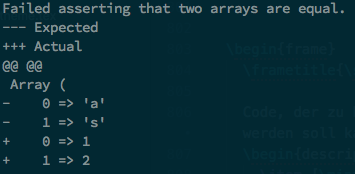
\includegraphics[width=0.75\textwidth]{assert-equals-array}
      \end{center}
    \end{figure}
  \end{block}
\end{frame}


\againframe<handout:0>{fragen}


\section{Fortgeschrittene Techniken}
\subsection{Template Methods}


\begin{frame}
  \frametitle{\subsecname}

  Code, der zu bestimmten Phasen des \alert{Lebenszyklus} eines Test ausgeführt werden soll kann in dazu vorgesehene Template-Methoden ausgelagert werden.
  \begin{description}[tearDownAfterClass()aaaaa]
    \item [\mintinline{php}|setUp()|] Wird vor jedem Test ausgeführt
    \item [\mintinline{php}|tearDown()|] Wird nach jedem Test ausgeführt
    \item [\mintinline{php}|setUpBeforeClass()|] Wird vor jedem TestCase ausgeführt
    \item [\mintinline{php}|tearDownAfterClass()|] Wird nach jedem TestCase ausgeführt
  \end{description}

\end{frame}


\begin{frame}[plain]

  \inputminted[firstline=10,lastline=30]{php}{composerExample/tests/Unit/ExamplePackage/MySecondExampleTest.php}

\end{frame}


\againframe<handout:0>{fragen}


\subsection{Data Provider}


\begin{frame}
  \frametitle{\subsecname}

  Will man in einem Test die Menge der \alert{Eingabeparameter und Resultate variieren} bieten sich \alert{Data Provider} an.
  Dataprovider können auch für mehrere Tests genutzt werden.

  \pause

  \begin{itemize}[<+->]
    \item Data Provider sind einzelne \alert{public Methoden}
    \item Data Provider geben ein \alert{Array von Parametern} zurück mit denen die Testmethode aufgerufen wird
    \item Die Verknüpfung von Methode und Data Provider wird mittels \alert{Annotation}
    hergestellt
  \end{itemize}

\end{frame}


\begin{frame}[plain]

  \inputminted[firstline=9,lastline=32]{php}{composerExample/tests/Unit/ExamplePackage/MyThirdExampleTest.php}

\end{frame}


\againframe<handout:0>{fragen}


\subsection{Exceptions}


\begin{frame}
  \frametitle{\subsecname}

  Unter gewissen Umständen möchte man, dass Methoden Exceptions werfen. Dieses verhalten lässt sich auch mit PHPUnit prüfen.

  \pause

  \begin{itemize}[<+->]
    \item Mittels Annotationen können Eigenschaften von \alert{Exceptions} asserted werden
    \item \mintinline{php}|@expectedException <Exception-Klasse>| legt die erwartete Klasse der Exception fest
    \item \mintinline{php}|@expectedExceptionCode <Code>| legt die erwartete Code fest
    \item \mintinline{php}|@expectedExceptionMessage <Message>| legt die erwartete Nachricht fest
  \end{itemize}

\end{frame}


\begin{frame}[plain]

  \inputminted[firstline=17,lastline=24,label=Quellcode]{php}{composerExample/src/ExamplePackage/MyThirdExample.php}

  \inputminted[firstline=34,lastline=45,label=Test]{php}{composerExample/tests/Unit/ExamplePackage/MyThirdExampleTest.php}

\end{frame}


\againframe<handout:0>{fragen}


\subsection{Output testen}


\begin{frame}
  \frametitle{\subsecname}

  PHPUnit ermöglicht es die \alert{Ausgabe einer Code-Unit} zu prüfen, die beispielsweise über \mintinline{php}{echo} oder \mintinline{php}{print} erzeugt werden. PHPUnit nutzt PHP's \alert{Output Buffering} um die Ausgabe abzufangen.

  \pause

  \begin{description}[<+->][expectOutputString()aaa]
    \item [\mintinline{php}{expectOutputString()}] erwartet, dass die Ausgabe nur aus dem übergebenen String besteht
    \item [\mintinline{php}{expectOutputRegex()}] erwartet, dass die Ausgabe auf die übergebenen Regex passt

  \end{description}

\end{frame}


\begin{frame}[plain,fragile]

  \inputminted[firstline=4,lastline=16,label=Quellcode]{php}{composerExample/src/ExamplePackage/MyFourthExample.php}

  \inputminted[firstline=7,lastline=17,label=Test]{php}{composerExample/tests/Unit/ExamplePackage/MyFourthExampleTest.php}

\end{frame}


\againframe<handout:0>{fragen}


\subsection{Mark test as \dots}


\begin{frame}
  \frametitle{\subsecname}

  PHPUnit bietet die Möglichkeit das \alert{Ergebnis eines Tests per Hand} zu setzen. Das ist besonders dann nützlich, wenn Tests unfertig sind, das Ergebnis eines Testlaufs trotzdem aussagekräftig sein soll.

  \pause

  \begin{description}[<+->][markTestIncomplete()aaa]
    \item [\mintinline{php}{markTestIncomplete()}] markiert einen Test als unvollständig. Optional kann eine Nachricht übergeben werden.
    \item [\mintinline{php}{markTestSkipped()}] lässt PHPUnit diesen Test überspringen. Optional kann eine Nachricht übergeben werden.
    \item [\mintinline{php}{fail()}] lässt den Test sofort fehlschlagen. Optional kann der Grund für den Fehlschlag übergeben werden.

  \end{description}

\end{frame}


\begin{frame}[fragile]
  \frametitle{\subsecname}

  \inputminted[firstline=7,lastline=17,highlightlines={11}]{php}{composerExample/tests/Unit/ExamplePackage/MyFifthExampleTest.php}

\end{frame}


\againframe<handout:0>{fragen}


\subsection{Hamcrest}


\begin{frame}
  \frametitle{\subsecname}

  \begin{block}{}
    \begin{quotation}
      Matchers that can be combined to create flexible expressions of intent.
    \end{quotation}
    \flushright{{\em -- \chref{http://hamcrest.org/}{hamcrest.org} }}
  \end{block}

  \pause

  \begin{itemize}[<+->]
  \item Detailierte Fehlerbeschreibung, wenn es keinen Match gibt
  \item Komplexe Strukturen mit einfachen Regeln matchen
  \item Matcher können wiederverwendet werden
  \item Alternative zu PHPUnit-asserts
  \item Flexibel im Aufbau
  \end{itemize}

\end{frame}


\begin{frame}[fragile]
  \frametitle{\subsecname}
  \framesubtitle{Fehlschlag}

  \inputminted[
    firstline=19,
    lastline=26,
    label=HamcrestTest.php
  ]{php}{composerExample/tests/Unit/ExamplePackage/HamcrestTest.php}

  \begin{figure}
    \centering
    Ausgabe
    \begin{minted}[label=Ausgabe,linenos=false]{php}
    Hamcrest\AssertionError : Expected: a string containing "bin kein"
       but: was "Ich bin ein string!"
    \end{minted}
  \end{figure}

\end{frame}


\begin{frame}
  \frametitle{\subsecname}
  \framesubtitle{Verschachtelung}

  \begin{itemize}[<+->]
    \item Jeder Parameter eines Matchers kann selbst wieder ein Matcher sein.
          \inputminted[
            firstline=28,
            lastline=37,
            label=HamcrestTest.php
          ]{php}{composerExample/tests/Unit/ExamplePackage/HamcrestTest.php}
    \item Auf diese Weise können Asserts \alert{präzise} und \alert{semantisch} im Code formuliert werden
  \end{itemize}
\end{frame}


\againframe<handout:0>{fragen}


\subsection{Mocks und Mockery}


\begin{frame}
  \frametitle{\subsecname}
  \begin{columns}
    \begin{column}{0.5\textwidth}
      \href{https://confluence.rdss.it/display/DEV/Workshop\%3A+Mockery?preview=/10683122/10683126/Mockery.handout.pdf}{
\includegraphics[width=0.9\textwidth]{cover-mockery}}
    \end{column}
    \begin{column}{0.5\textwidth}
      Zu diesem Thema gab es bereits einen Vortrag. Die Unterlagen finden sich in unserem Wiki.
      \vspace*{1em}
      \href{https://confluence.rdss.it/display/DEV/Workshop\%3A+Mockery?preview=/10683122/10683126/Mockery.handout.pdf}{\beamergotobutton{Mockery-Präsentation}}
    \end{column}
  \end{columns}

\end{frame}


\section{Komplexes Beispiel}


\begin{frame}
  \frametitle{\secname}

  \begin{figure}
    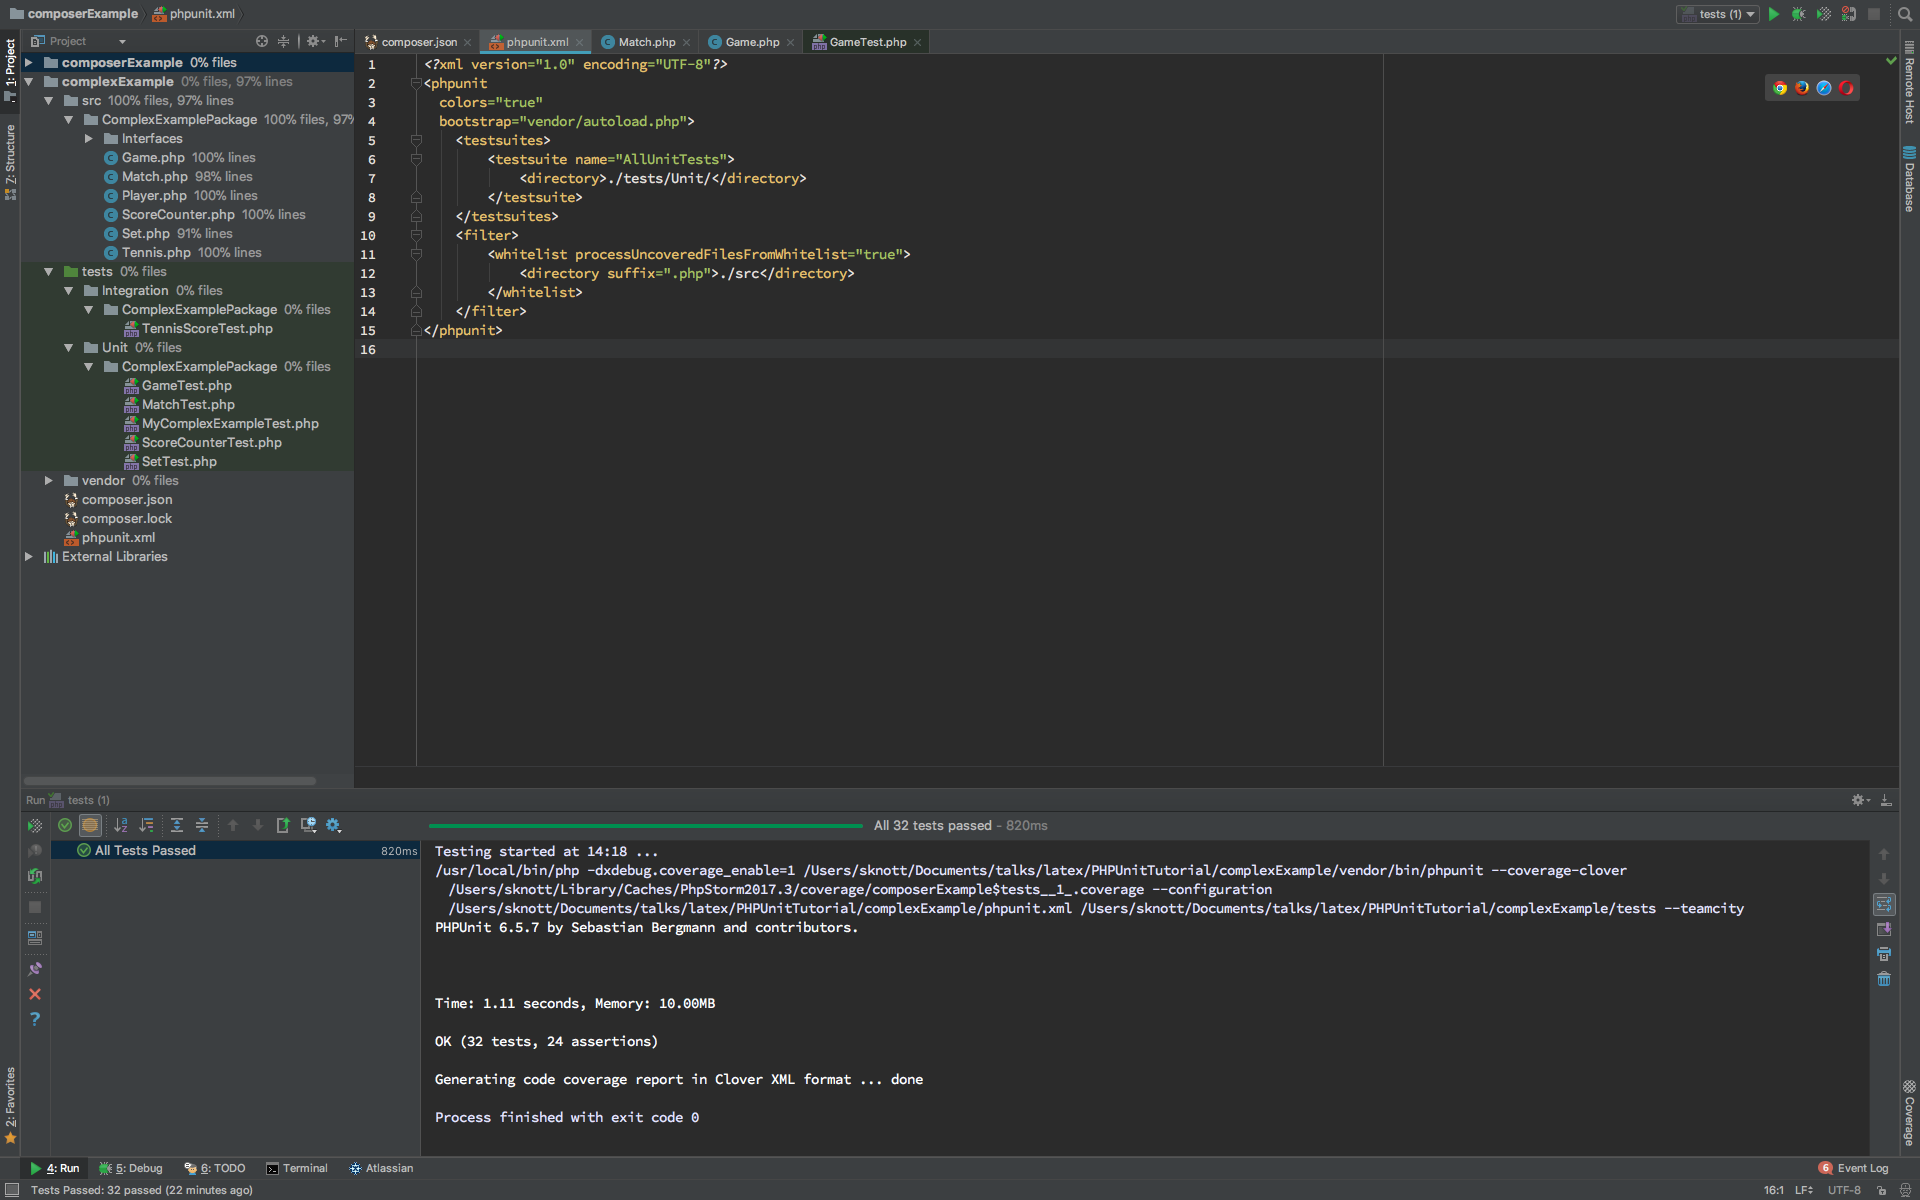
\includegraphics[width=\textwidth]{Images/phpstorm-komplexes-beispiel}
  \end{figure}

\end{frame}


\againframe<handout:0>{fragen}


\section{Code Dojo}


{
\usebackgroundtemplate{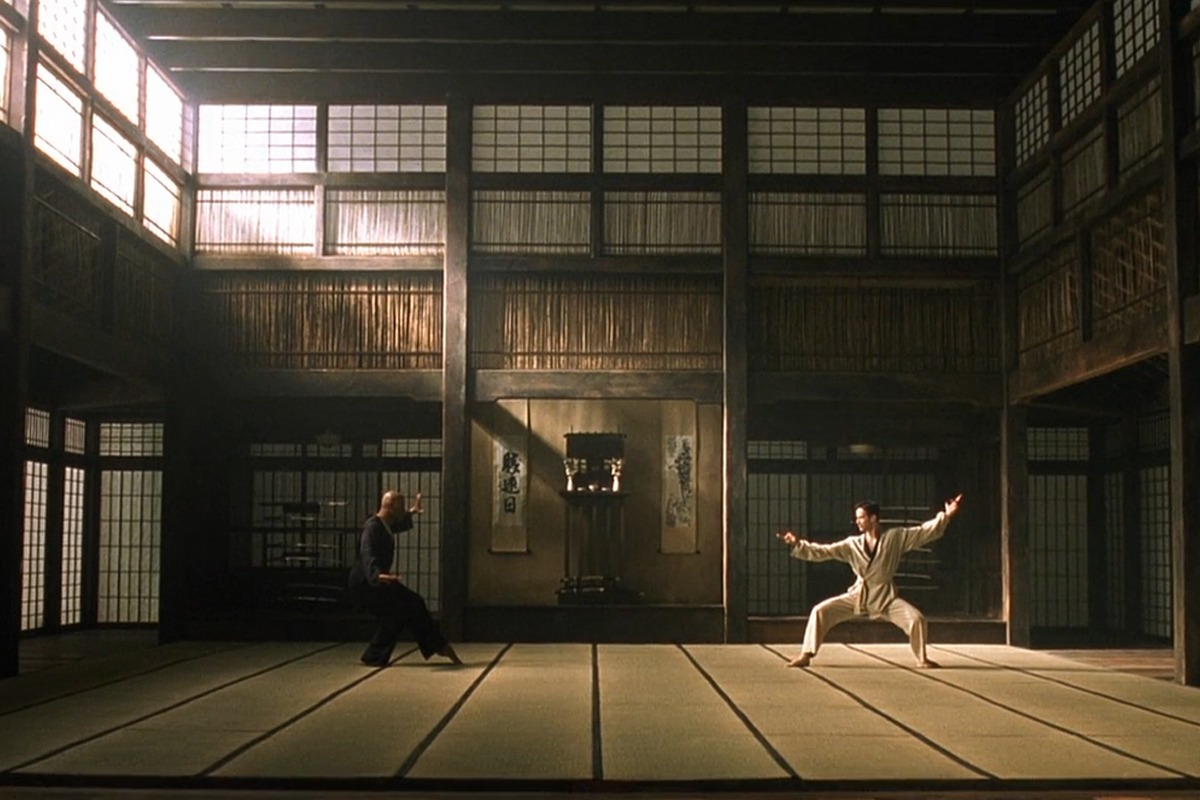
\includegraphics[height=\paperheight,width=\paperwidth]{dojo}}
\setbeamertemplate{blocks}[rounded][shadow=false]

  \begin{frame}[fragile]
    \frametitle{Code Dojo}
    \framesubtitle{Was ist ein Dojo?}
    \begin{exampleblock}{}
      Dojo (jap. Ort des Weges) bezeichnet einen Trainingsraum für verschiedene japanische Kampfkünste (Budo) [\dots]. Im übertragenen Sinne steht der Begriff auch für die Gemeinschaft der dort Übenden.
      \flushright{{\em -- Wikipedia}}
    \end{exampleblock}
  \end{frame}


  \begin{frame}[fragile]
    \frametitle{Code Dojo}
    \framesubtitle{Was ist ein Dojo?}

    \begin{exampleblock}{}
      Die Gemeinschaft führt gemeinsam Übungen -- so genannte Katas -- durch um ihr Wissen in der entsprechenden Disziplin zu vervollkommnen.
    \end{exampleblock}
  \end{frame}
}


\begin{frame}[fragile]
  \frametitle{Code Kata}
  \framesubtitle{Was ist ein Code Kata?}

  \begin{figure}
    \begin{center}
      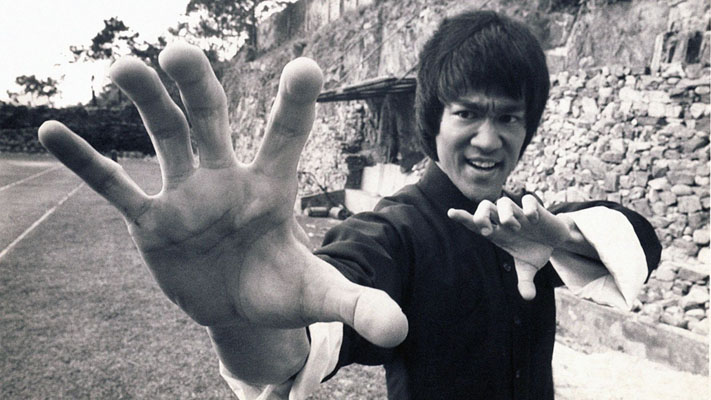
\includegraphics[width=0.7\textwidth]{bruce-lee}
    \end{center}
  \end{figure}

  \begin{itemize}
    \item<+-> Kleine, unabhängige, fokussierte, in sich geschlossene Übung
    \item<+-> Übt die Ausführung und Herangehensweise
    \item<+-> Bietet Raum für gemeinsames Lernen
    \item<+-> Lösung der Aufgabe erklärtes Nicht-Ziel
  \end{itemize}

\end{frame}


{
\usebackgroundtemplate{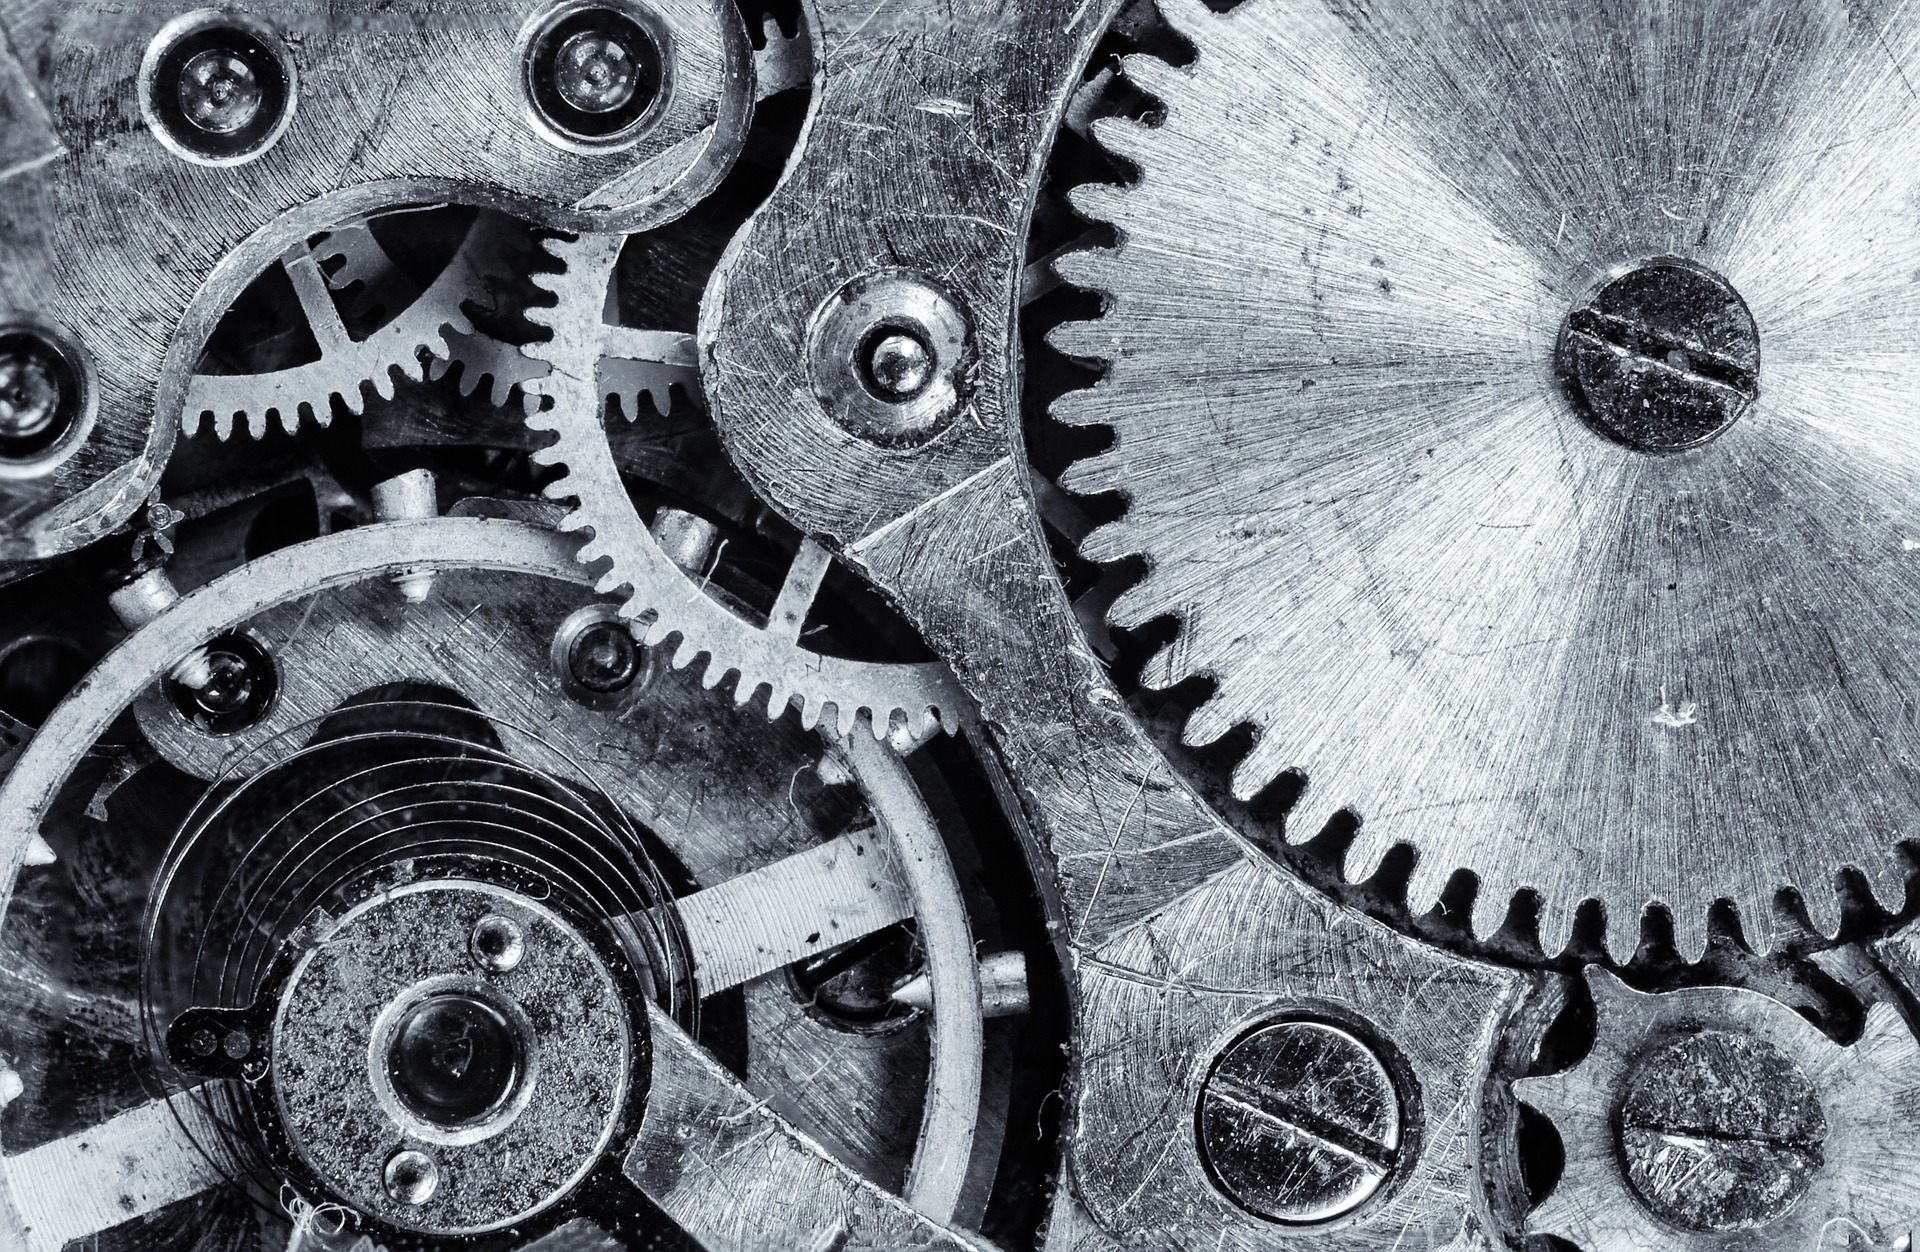
\includegraphics[height=\paperheight,width=\paperwidth]{gears}}
\setbeamertemplate{blocks}[rounded][shadow=false]

\begin{frame}[fragile]
  \frametitle{Das Tennis Kata}
  \framesubtitle{Fokus}
  \begin{block}{Fokus}
    \begin{itemize}
      \item<+-> Pair Programming + TDD = TDD-Game
      \item<+-> Keine PHPMD Regel darf gebrochen werden
      \item<+-> Absichtsvolles Testen
      \begin{itemize}
        \item<+-> Test wird zuallererst dem Pair-Partner erklärt, dann programmiert
        \item<+-> Auswahl des Zwecks (use case, Erwartete Eingaben \dots)
        \item<+-> Auswahl der Kategorie (Black-, White-box)
        \item<+-> Gegebenenfalls Auswahl der Äquivalenzklasse.
      \end{itemize}
    \end{itemize}
  \end{block}

\end{frame}
}


{
\usebackgroundtemplate{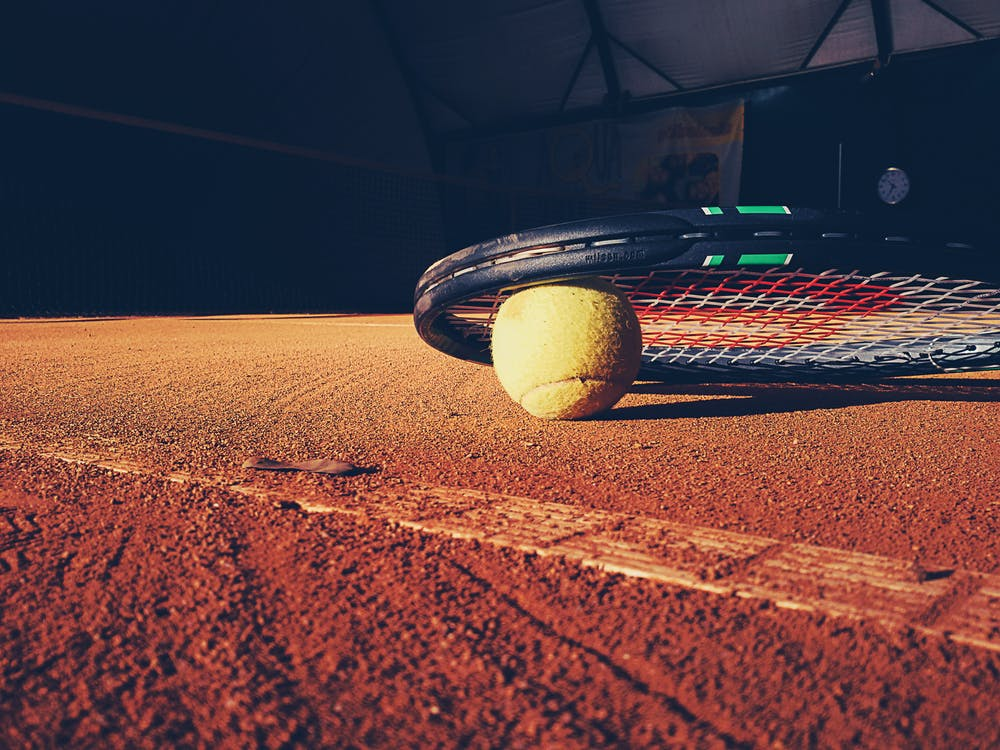
\includegraphics[width=\paperwidth]{tennis.jpg}}
\setbeamertemplate{blocks}[rounded][shadow=false]

\begin{frame}[fragile]

  \frametitle{Das Tennis Kata}
  \framesubtitle{Anforderung}

  \begin{block}{Anforderung}
    \begin{itemize}
      \item Eine Klasse muss die folgenden public Methoden haben
      \begin{itemize}
        \item \highlighton{addPointToPlayer(player:PlayerInterface):null} - Soll aufgerufen werden wenn ein Spieler einen Punkt erzielt. Wirft eine Exception, wenn das Spiel vorbei ist
        \item \highlighton{getScore():string} - Gibt eine Übersicht über alle gespielten Sätze, den aktuellen Punktestand und ob ein Spieler gewonnen hat aus.
        Es gelten die \href{https://de.wikipedia.org/wiki/Tennis#Gliederung_und_Zählweise}{Tennisregeln} mit 2 Gewinnsätzen.
      \end{itemize}
    \end{itemize}
  \end{block}

\end{frame}
}

%-------------------------------------------------------
% HELPER PAGES
%-------------------------------------------------------

\appendix

\begin{frame}<handout:0>[label=5minPause]
  \frametitle{Pause}
  \framesubtitle{5 Minuten Pause}
  \begin{figure}
    \begin{center}
      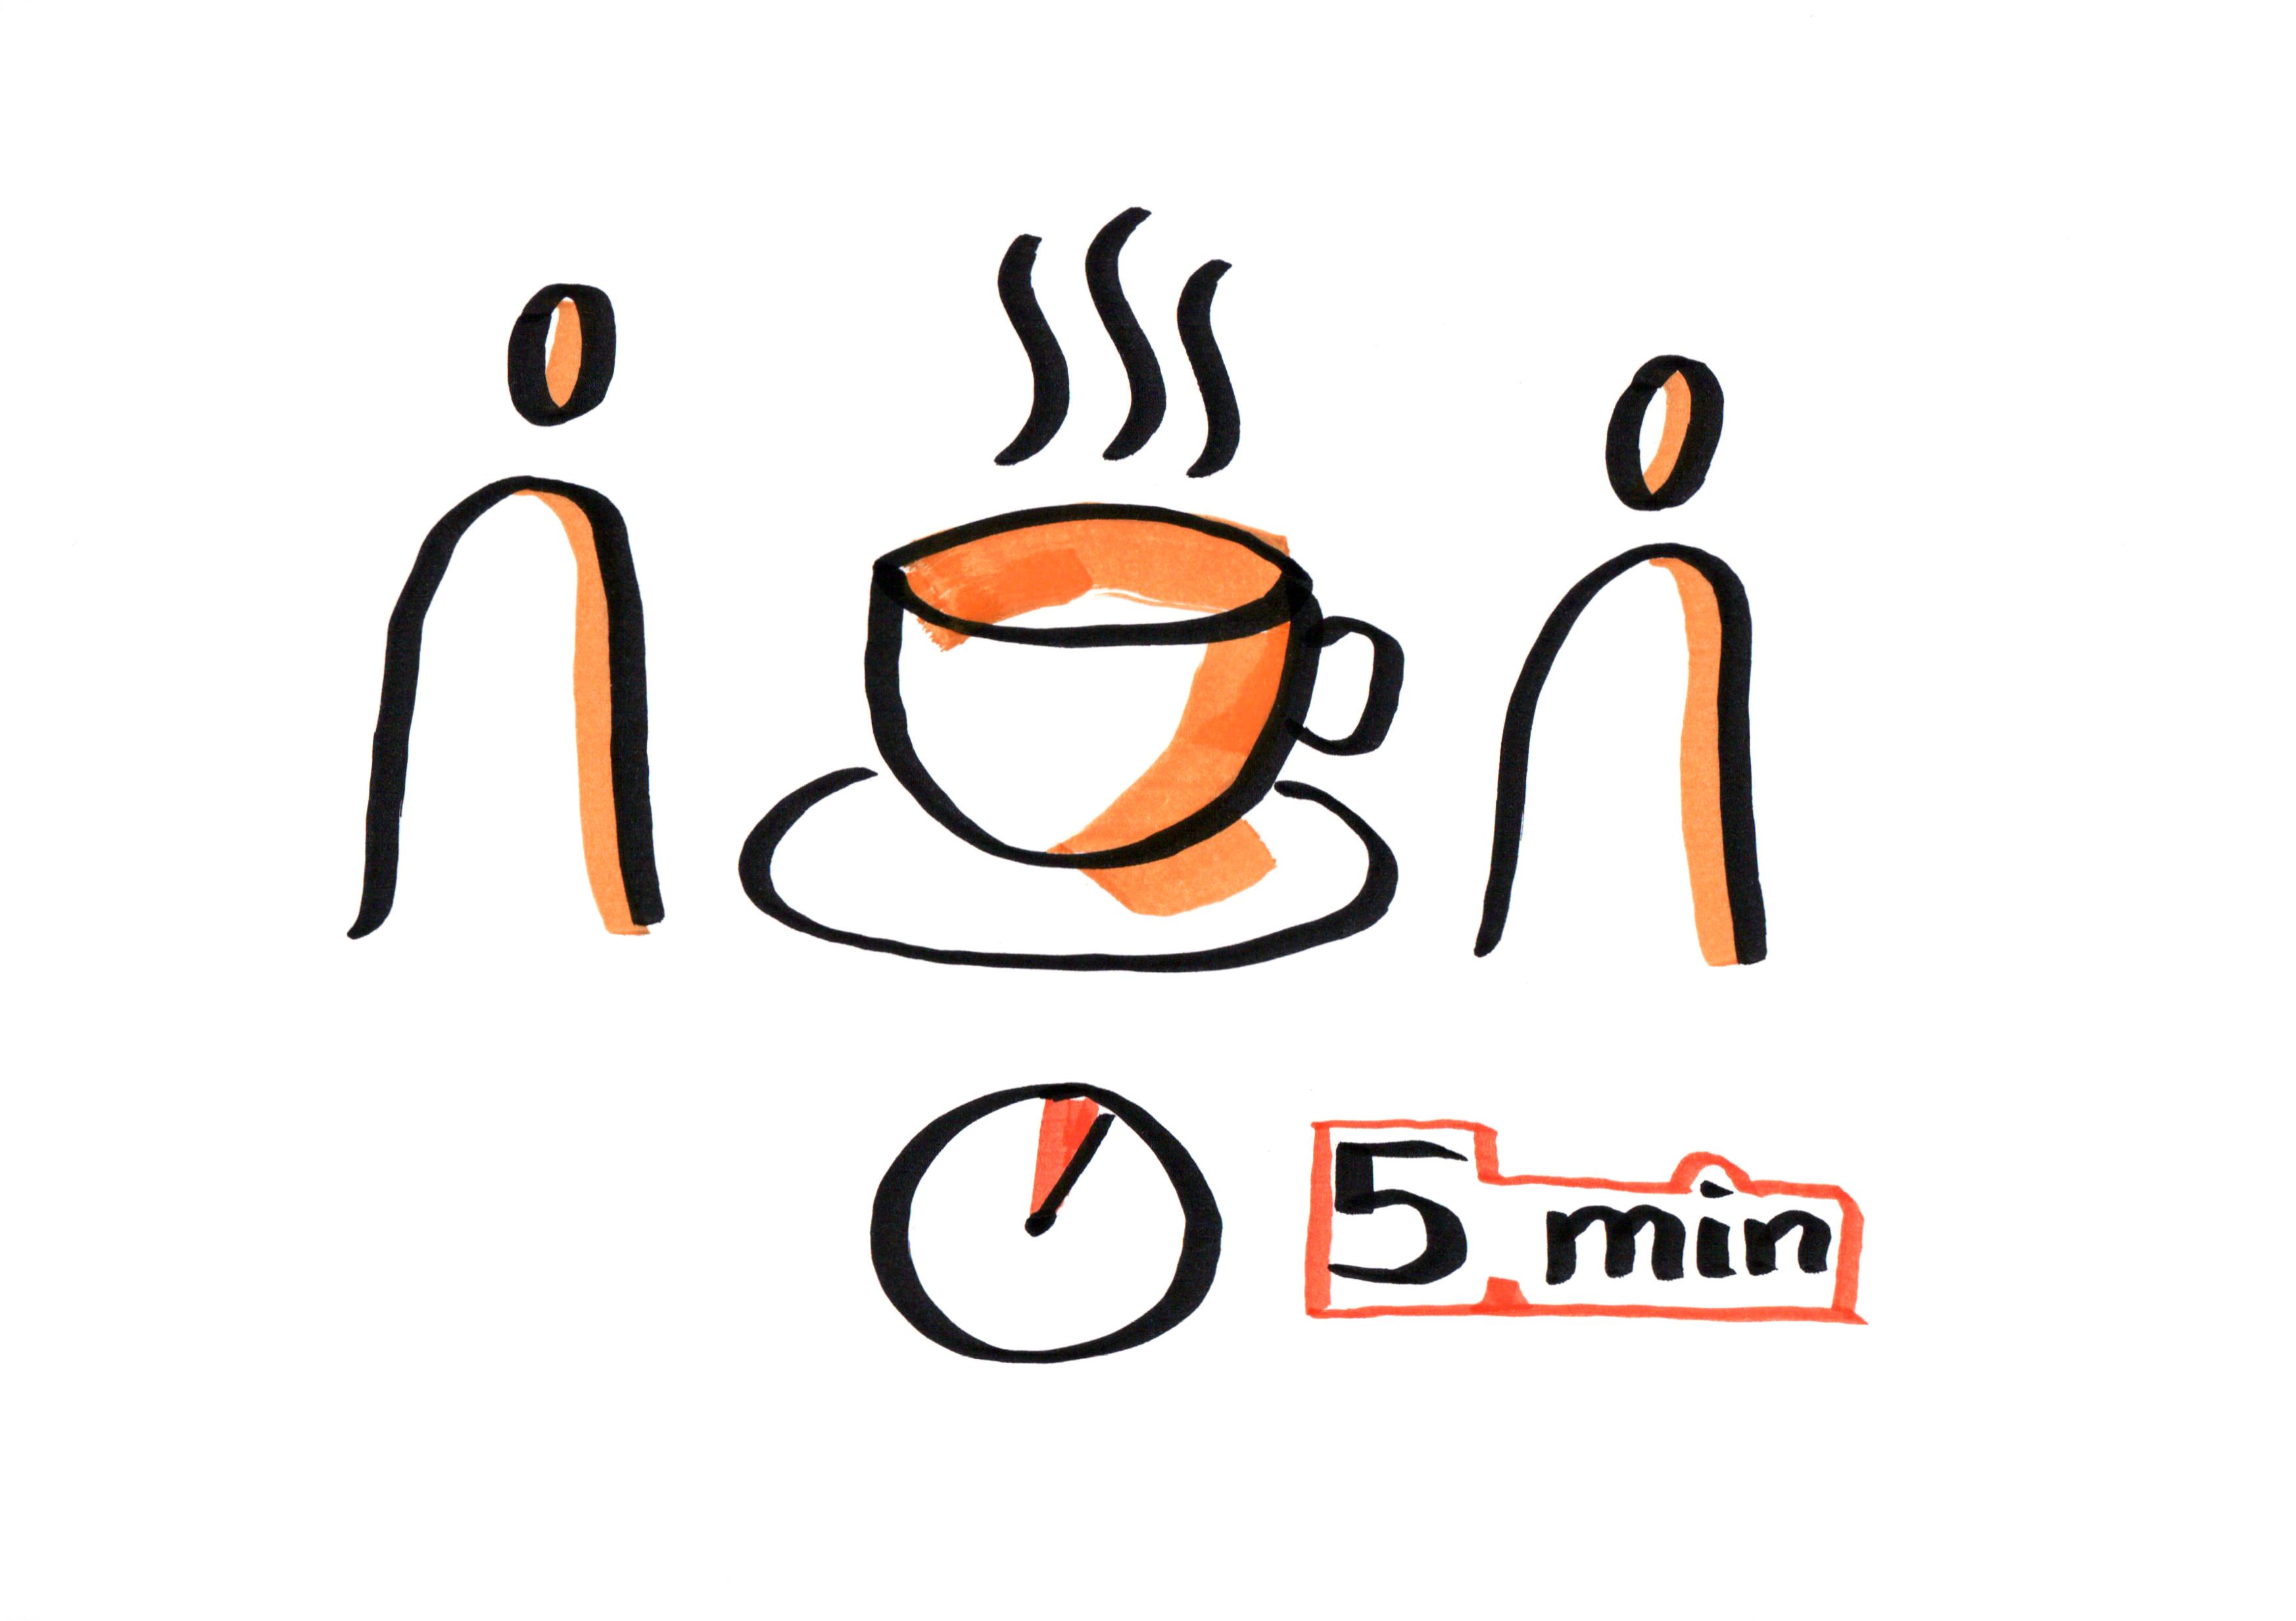
\includegraphics[height=4cm]{pause-5-min}
    \end{center}
  \end{figure}
\end{frame}



\begin{frame}<handout:0>[label=10minPause]
  \frametitle{Pause}
  \framesubtitle{10 Minuten Pause}
  \begin{figure}
    \begin{center}
      
\includegraphics[height=4cm]{pause-10-min}
    \end{center}
  \end{figure}
\end{frame}



\begin{frame}<handout:0>[label=pause]
  \frametitle{Pause}
  \framesubtitle{Pause}
  \begin{figure}
    \begin{center}
      
\includegraphics[height=4cm]{pause}
    \end{center}
  \end{figure}
\end{frame}



\begin{frame}<handout:0>[label=fragen,fragile]
  \frametitle{Fragen}
  \framesubtitle{Fragen?}
  \begin{figure}
    \begin{center}
      
\includegraphics[height=4cm]{fragen}
    \end{center}
  \end{figure}
\end{frame}



\end{document}

\end{document}
